In this chapter, methodologies to address the long-tail issue and the challenge of temporal redundancy are explored. Afterwards, a detailed explanation of the Transformer-based video backbone and multi-modality contrastive learning, which are fundamental to this research, is provided.

\section{Addressing the Long-Tail Issue}
In previous research, three main groups of strategies have been employed to deal with the long-tail issue: Re-weighting, Re-sampling, and Few-Shot Learning.

\subsection{Re-weighting}
Re-weighting is a technique used to adjust the penalties for specific groups of classes or samples. This is typically achieved by modifying the loss function. The most vanilla re-weighting scheme involves applying the inverse class frequency to the loss. In this manner, more frequent classes receive a lower weight of loss, enabling the model to put more emphasis on the tail classes \parencite{khan2017cost, mostajabi2015feedforward}.

However, it has been proved that as the number of samples increases, the marginal benefit of model performance diminishes. As a result, directly applying the inverse class frequency to the loss function may overly reduce the weight of losses for the frequent classes. To address this, the Class Balanced Loss (CB Loss) was introduced. As illustrated in Figure \ref{fig:concetpcbloss}, CB Loss calculates the effective number of samples to balance the inverse class frequency, yielding a more reasonable weight for the loss \parencite{cui2019class}.

\begin{figure}[ht]
    \centering
    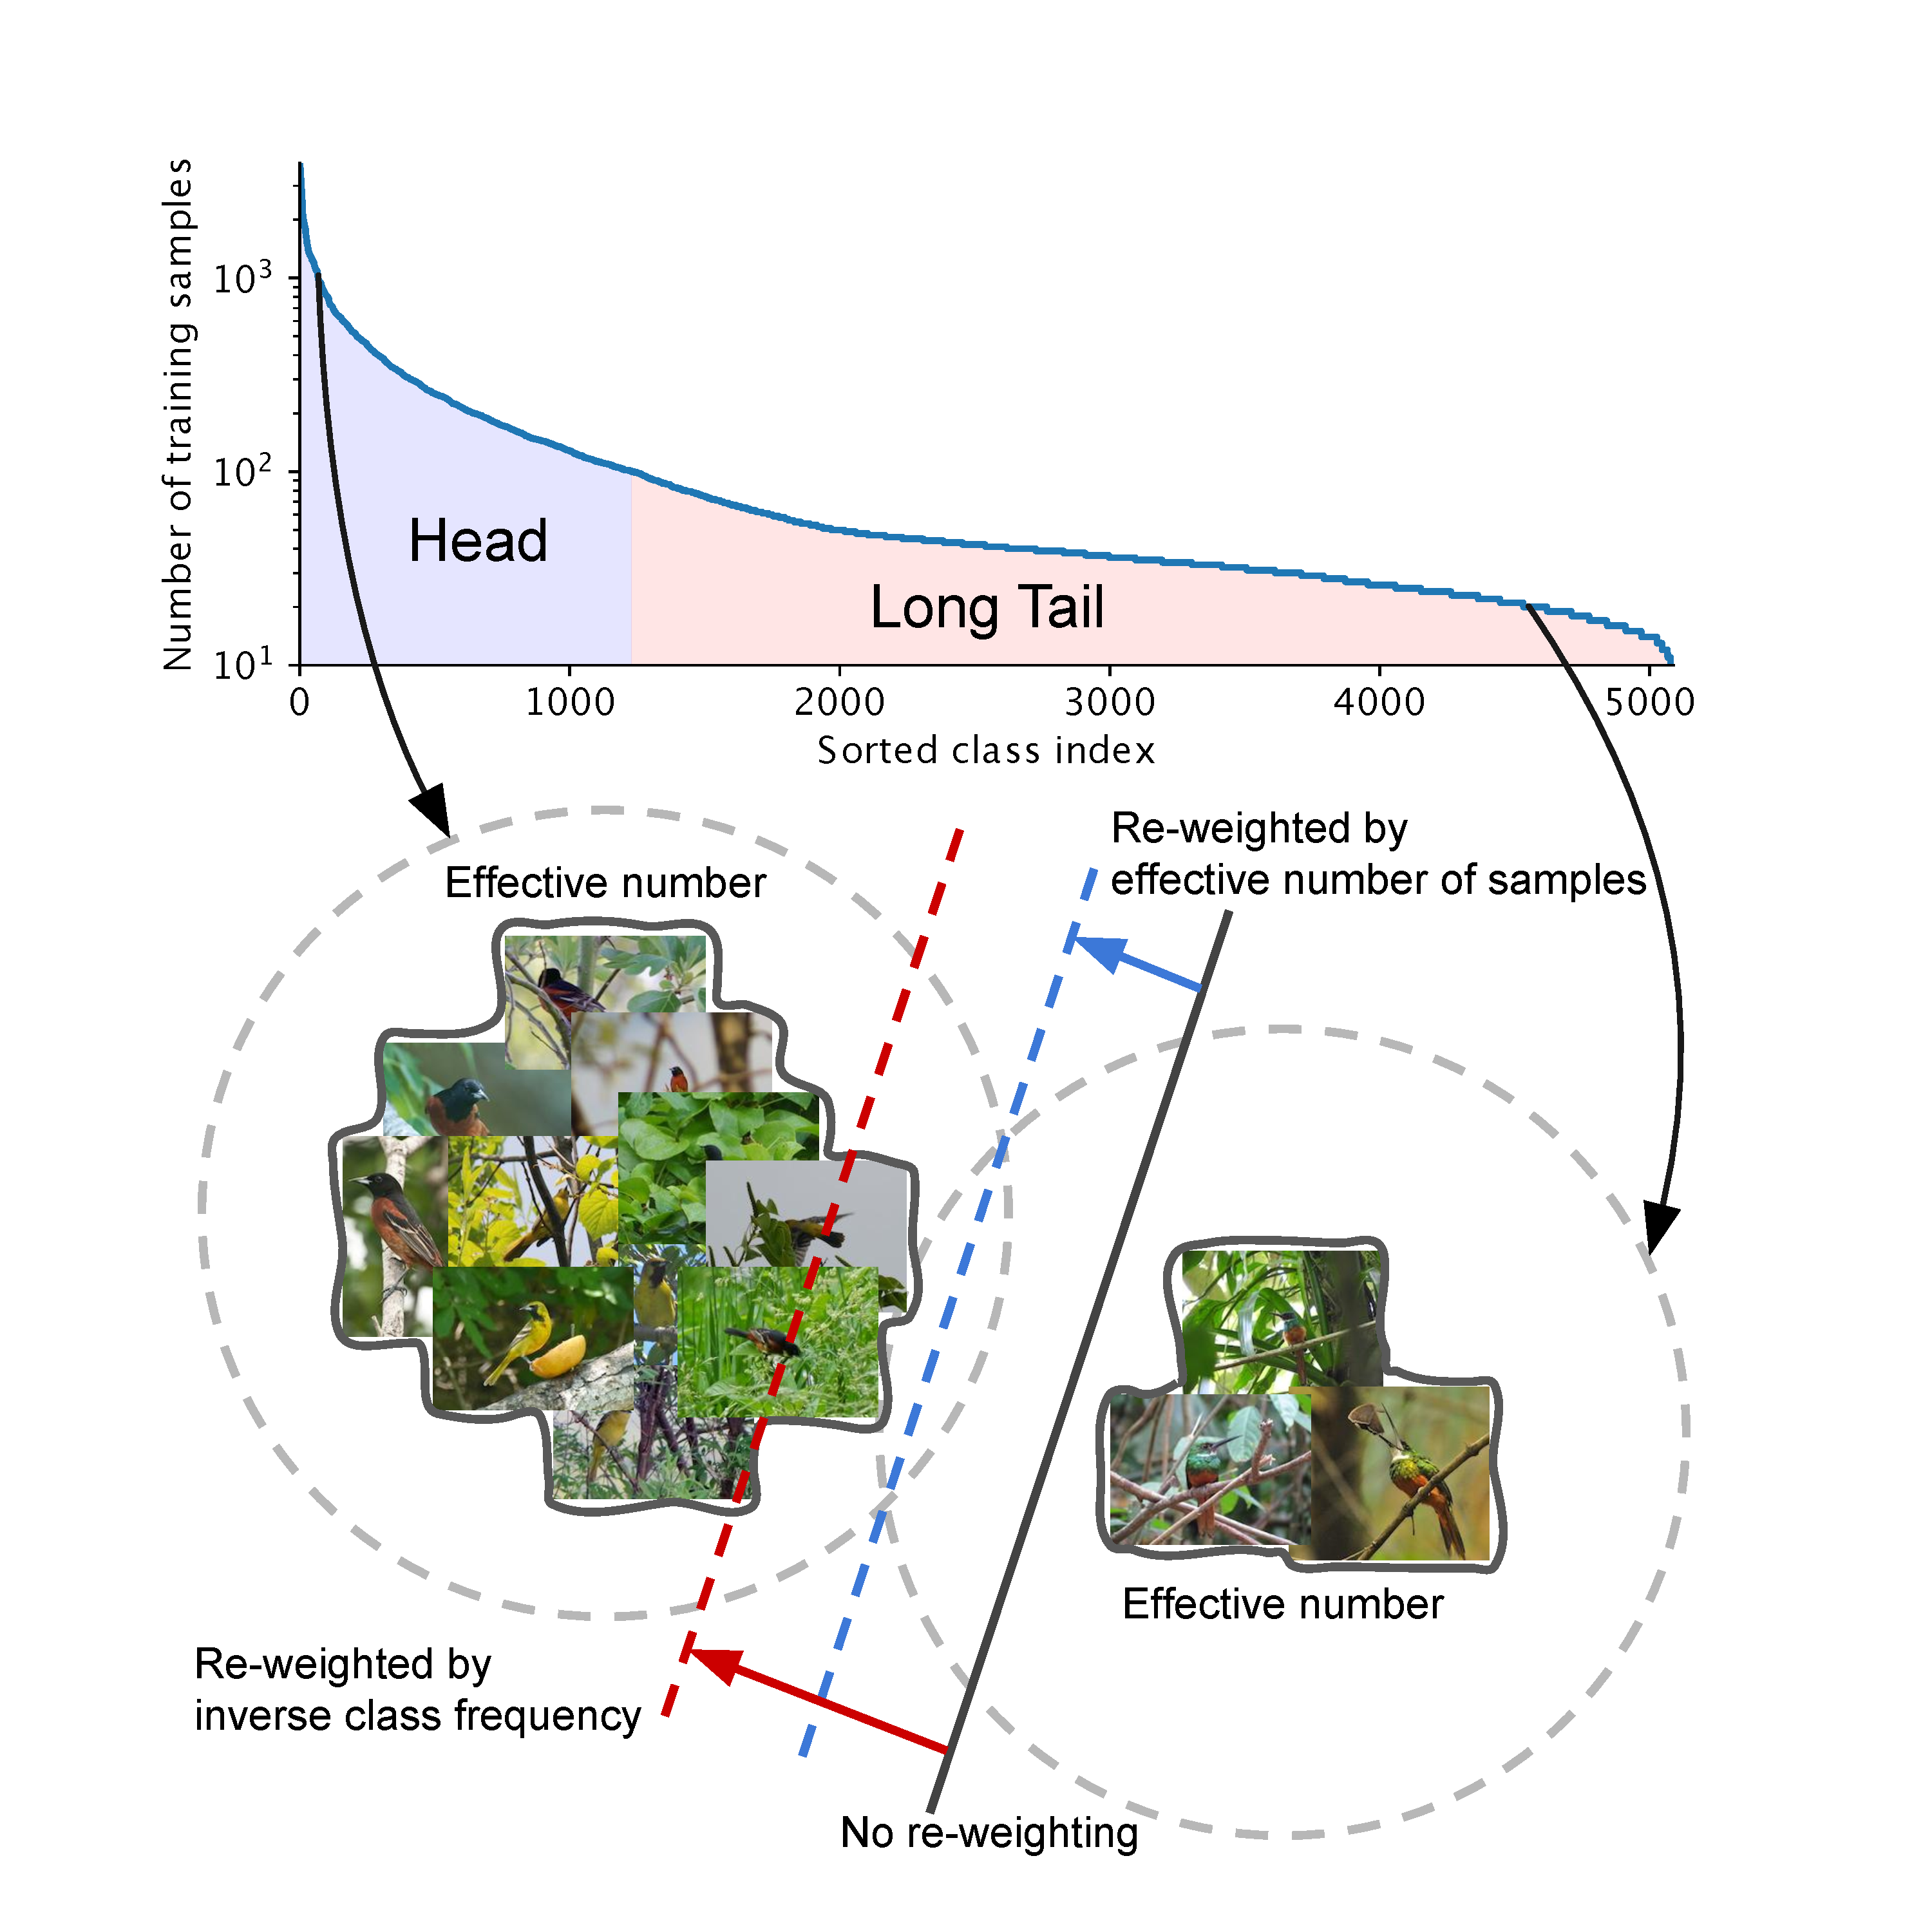
\includegraphics[width=0.5\textwidth]{assets/charts_rw/CBLoss}
    \caption[Conceptual Illustration of CB Loss]{This figure illustrates the concept of CB Loss. provides a visual representation of the CB Loss concept, where the effective number of samples is computed for re-weighting purposes. Source: \parencite{cui2019class}}
    \label{fig:concetpcbloss}
\end{figure}

In contrast to frequency-based re-weighting, Focal Loss focuses on the difficulty level of learning. It scales the penalty to automatically down-weight the contribution of easy examples, which enforces the model to focus more on the hard examples \parencite{lin2017focal}.

The Label-Distribution-Aware Margin (LDAM) Loss, inspired by the hinge loss of Support Vector Machine, ensures that the model establishes a closer decision boundary while classifying frequent classes, as illustrated in Figure \ref{fig:concetpldam}, to provide room for the less frequent class with more uncertainty. This implies that the model is required to produce higher confidence probabilities to achieve a better performance \parencite{cao2019learning}.

\begin{figure}[ht]
    \centering
    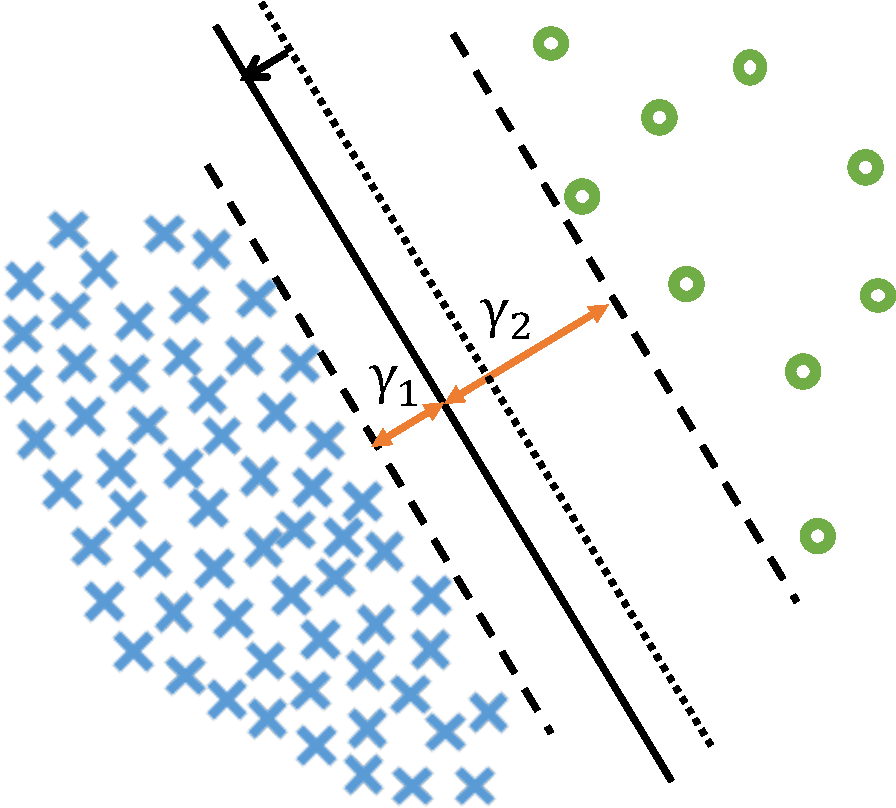
\includegraphics[width=0.5\textwidth]{assets/charts_rw/LDAM}
    \caption[Conceptual Illustration of LDAM]{This figure illustrates the LDAM concept, where the decision boundary is adjusted toward the frequent classes to provide room for the less frequent class with more uncertainty. Source: \parencite{cao2019learning}}
    \label{fig:concetpldam}
\end{figure}

In the context of videos, re-weighting may not be the best strategy to overcome the long-tail issue. Considering the varying amounts of information in a single video, adjusting the weights to tail classes is likely to introduce noise into the training process \parencite{zhang2021videolt}.

\subsection{Re-sampling}
Re-sampling refers to the intuitive use of sampling algorithms to balance the number of samples for each class. Several early research studies have applied this technique to enhance the model performance \parencite{shen2016relay, 5128907, mahajan2018exploring}.

Previous research has also found that data imbalance itself does not affect the performance of representation learning. Although re-sampling has led to better performance in classification results, it actually benefits classifier learning while harming representation learning. Consequently, subsequent research has focused more on re-sampling techniques used in classifier training \parencite{zhou2020bbn, kang2019decoupling}.

Compared to the previous method that focused on re-sampling algorithms, subsequent research has attempted to reconstruct more samples. For instance, VideoLT concatenates frames from different videos to generate additional tail samples \parencite{zhang2021videolt}. Similarly, reconstruction of samples in the embedding space has also been explored by researchers \parencite{liu2022long, perrett2023use}. For example, Long-Tail Mixed Reconstruction \parencite{perrett2023use}, as illustrated in Figure \ref{fig:augembedding}, decomposes the entire model into image encoder and classifier and reconstructs samples using the embeddings generated by the image encoder.

\begin{figure}[ht]
    \centering
    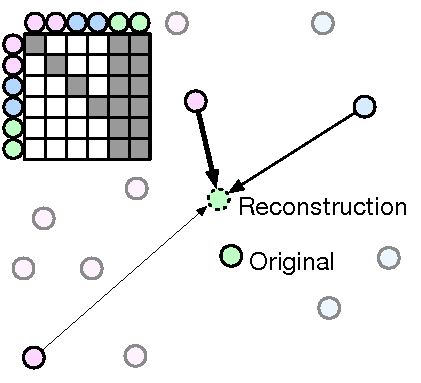
\includegraphics[width=0.5\textwidth]{assets/charts_rw/AugEmbedding}
    \caption[Illustration of Reconstruction of Samples in the Embedding Space]{This chart illustrates the concept of reconstructing samples in the embedding space. Tail samples, represented in green, are reconstructed from other batch samples using the weighted sum method. row-axis samples of the top-left matrix in the figure denote the features to be reconstructed, while column-axis samples are the features being used for the reconstruction. Grey-highlighted cells are masked out for the weighted sum calculation. Source: \parencite{perrett2023use}}
    \label{fig:augembedding}
\end{figure}

These re-sampling techniques certainly mitigate poor performance in the tail classes. Nevertheless, they do not guarantee the production of samples to have the same variety and correctness as the collected data.

\subsection{Few-Shot Learning}
Recent research has increasingly focused on learning techniques that require fewer training data to achieve acceptable performance.

Model-Agnostic Meta-Learning (MAML) \parencite{finn2017model} introduced the concept of learning to initialise better parameters for training. This innovation has led to a series of studies on meta-learning. Apart from initialisation \parencite{nichol2018first, 2018Reptile}, a large amount of research has emerged, applying meta-learning to various aspects, such as optimization technique search \parencite{andrychowicz2016learning}, data augmentation strategies \parencite{li2020dada, galashov2022data, cubuk2018autoaugment}, and even re-weighting strategies \parencite{shu2019meta}. For example, Figure \ref{fig:concetpdada} illustrates the concept of Differential Automation Data Augmentation (DADA) \parencite{li2020dada}, which presents a differentiable approach to image augmentation for meta-learning.

\begin{figure}[ht]
    \centering
    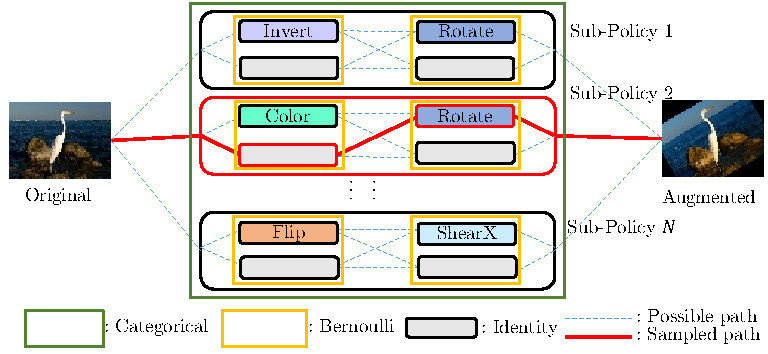
\includegraphics[width=0.8\textwidth]{assets/charts_rw/DADA}
    \caption[Illustration of Differential Automation Data Augmentation]{This figure illustrates the concept of Differential Automation Data Augmentation. Source: \parencite{li2020dada}}
    \label{fig:concetpdada}
\end{figure}

With the capability to learn from small datasets, few-shot learning techniques also mitigate the long-tail issue. MetaModelNet, for example, regresses the parameters from models trained with fewer data to those trained with more \parencite{NIPS2017_147ebe63}. Moreover, some studies have indicated that augmentation or memory retrieval in the embedding space are effective ways to handle tail classes \parencite{liu2019large, Zhu_2020_CVPR, li2021metasaug, Fu_2022_ACCV}.

These approaches primarily focus on few-shot learning or generalising the representation learned from the head classes to the tail classes. In contrast,  CLIP \parencite{radford2021learning} embeds both images and text into a unified semantic space, as shown in Figure \ref{fig:clipstructure}. This empowers the model to effectively leverage human intelligence to understand visual data and balance the distribution of learning targets \parencite{ma2022x}. 

\begin{figure}[ht]
    \centering
    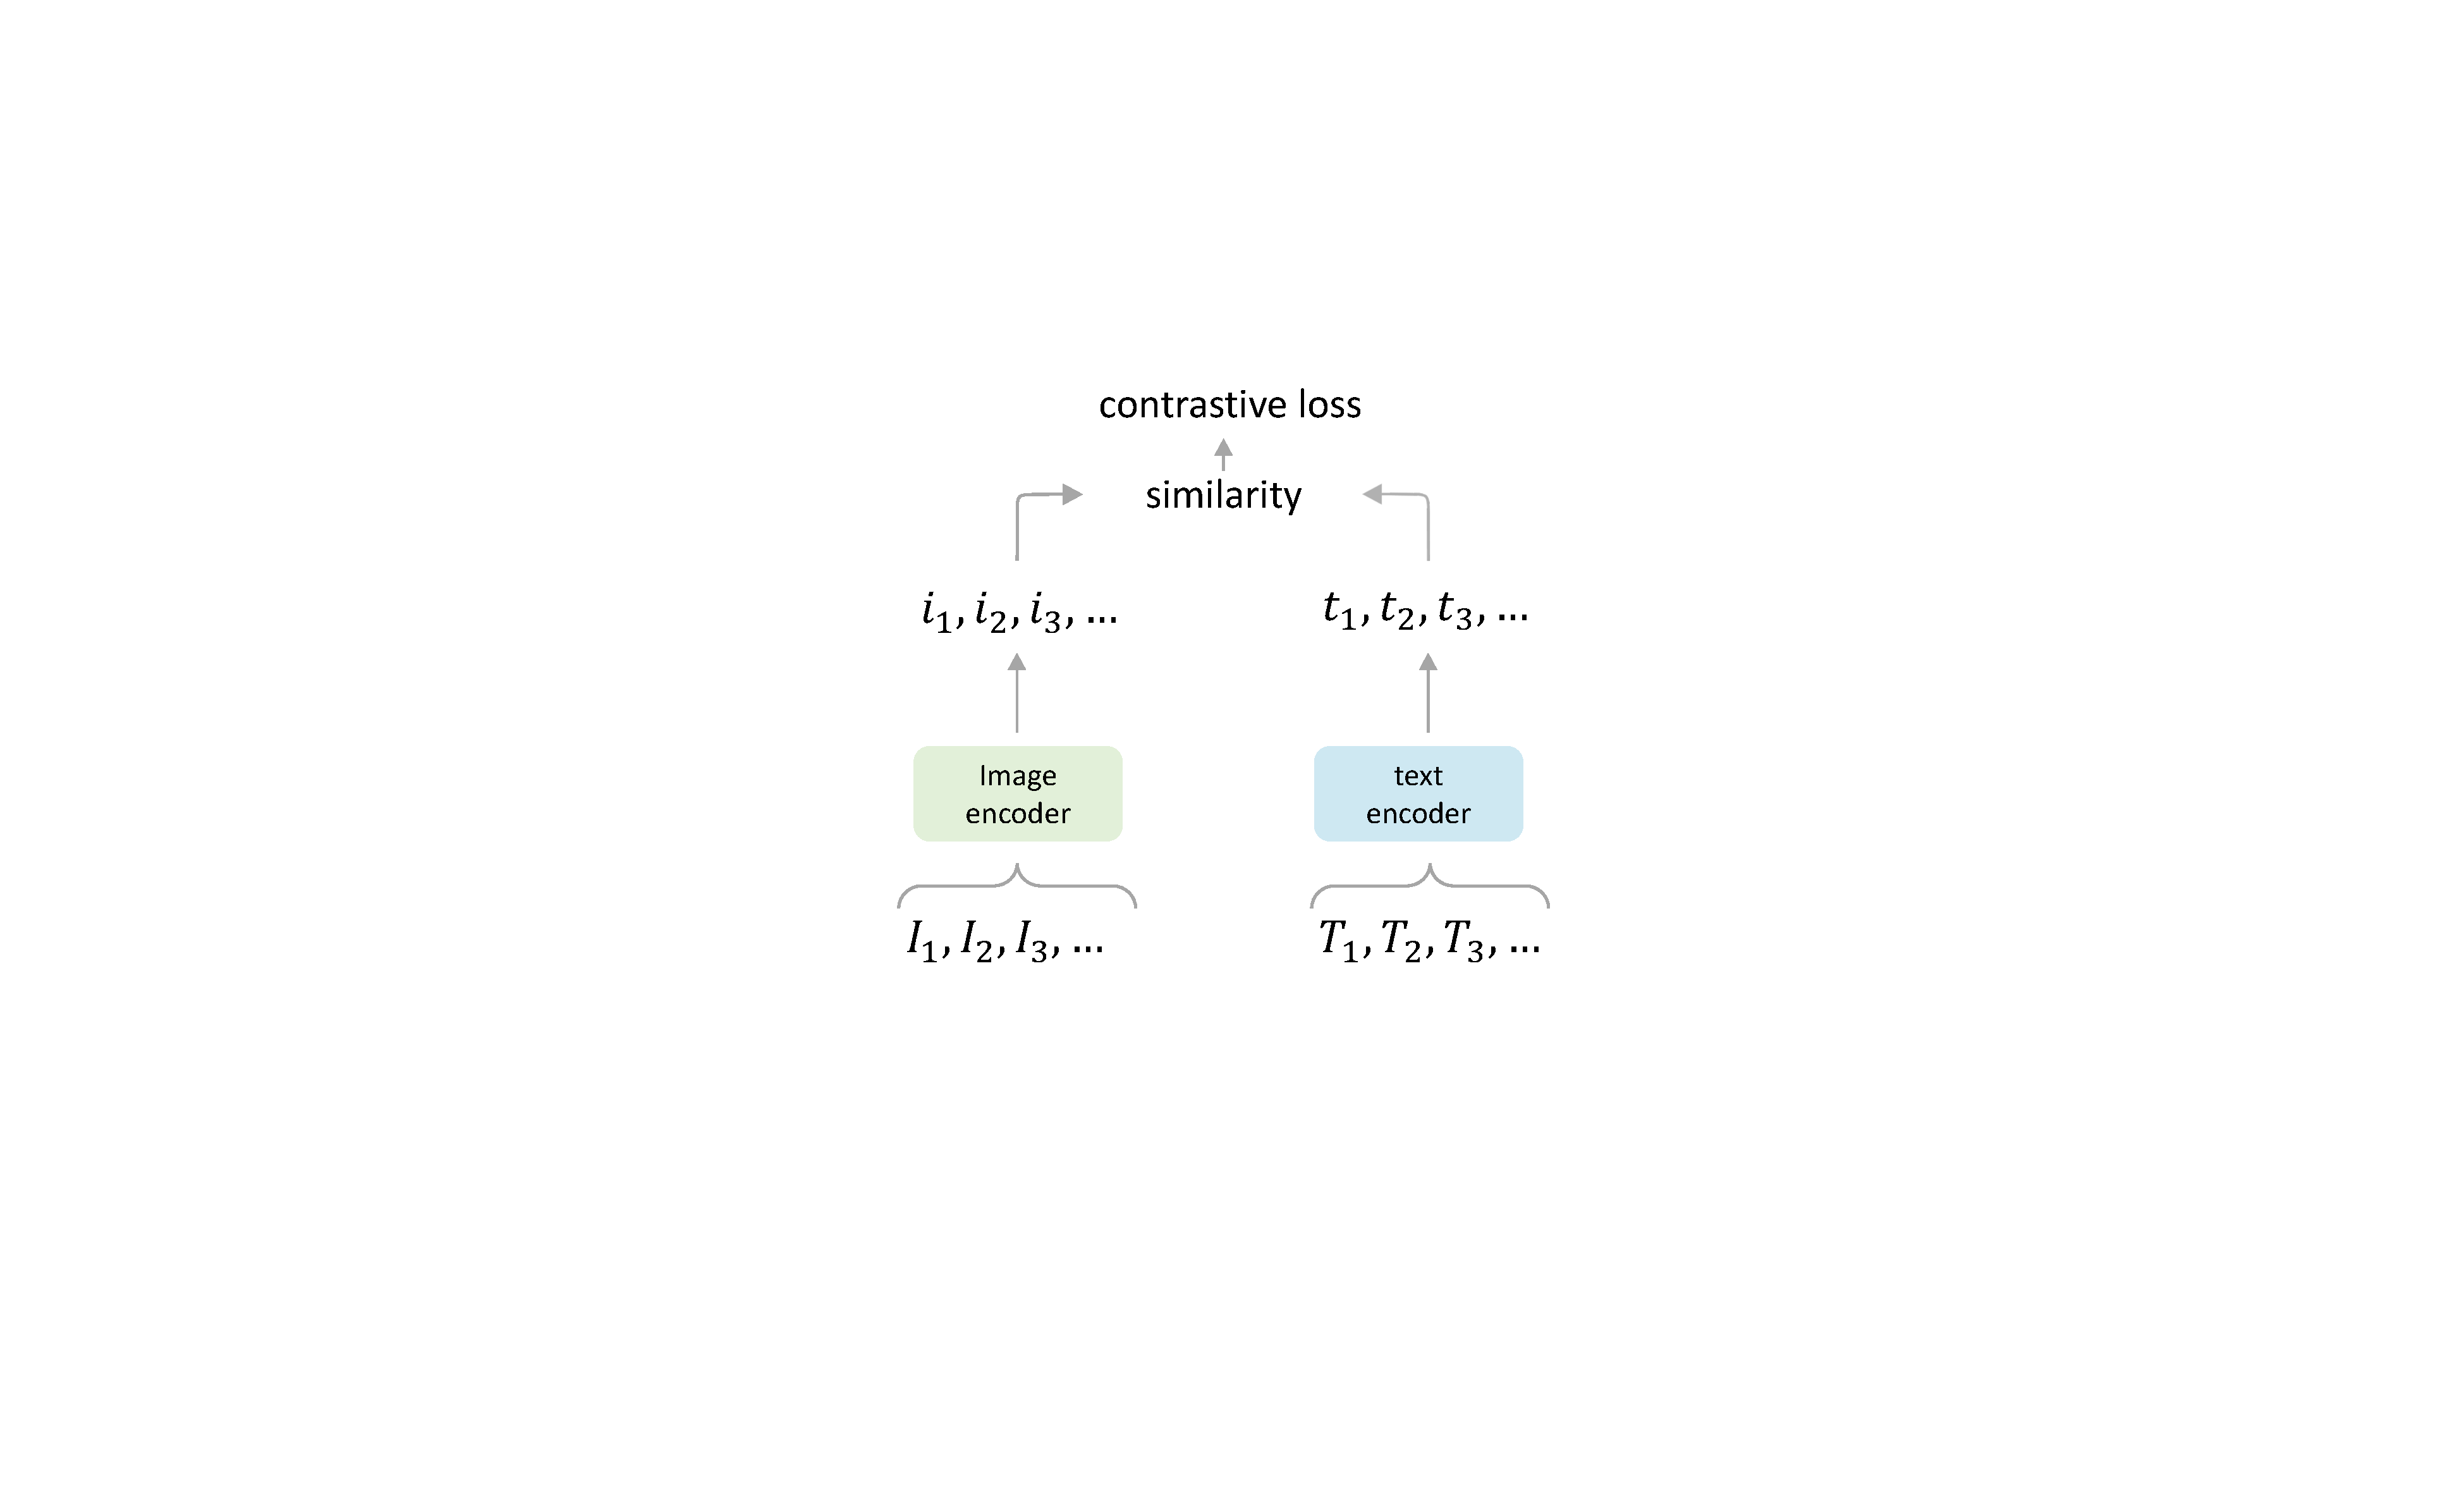
\includegraphics[width=0.5\textwidth]{assets/charts_rw/CLIP}
    \caption[Illustration of CLIP Model Structure]{This figure illustrates the structure of the CLIP model. The left stream encodes images, while the right stream encodes text. Both streams are embedded into the same semantic space. Source: \parencite{cui2022contrastive}}
    \label{fig:clipstructure}
\end{figure}

With these advantages, CLIP has been applied to several image downstream tasks including few-shot learning \parencite{zhang2022tip}, segmentation \parencite{wang2022cris}, video retrieval \parencite{ma2022x}, object detection \parencite{lin2023gridclip}, and captioning \parencite{mokady2021clipcap}. In addition, CLIP for videos has also been proposed \parencite{xu-etal-2021-videoclip, wang2022internvideo}, achieving state-of-the-art results in several video downstream tasks such as classification, video retrieval, and vision question answering.

This research focuses on the long-tail issue and has demonstrated that the text encoder of pretrained CLIP is an efficient tool to tackle the scarcity problem of tail classes.

\section{Temporal Redundancy}
Boundaries of objects in frames and small displacements between neighbouring frames have been identified as significant features for action recognition \parencite{10.1007/978-3-030-12939-2_20}. In order to enhance the model in this aspect, optical flow and pretext learning are two research directions. 

\subsection{Optical Flow}
To capture subtle boundary changes between frames, the integration of optical flow as an independent stream within model structures has become a popular strategy for action recognition \parencite{sevilla2019integration, tran2015learning, carreira2017quo}. For instance, the I3D architecture \parencite{carreira2017quo} utilizes a 3D CNN on both the RGB and optical flow stream, whose outputs are subsequently summed together to generate the final prediction. This is showcased in subfigure (e) of Figure \ref{fig:structuresi3d}. As Figure \ref{fig:structuresi3d} illustrates, it compares its structure to other four networks, two of which also incorporate optical flow as an independent stream for action recognition.

\begin{figure}[ht]
    \centering
    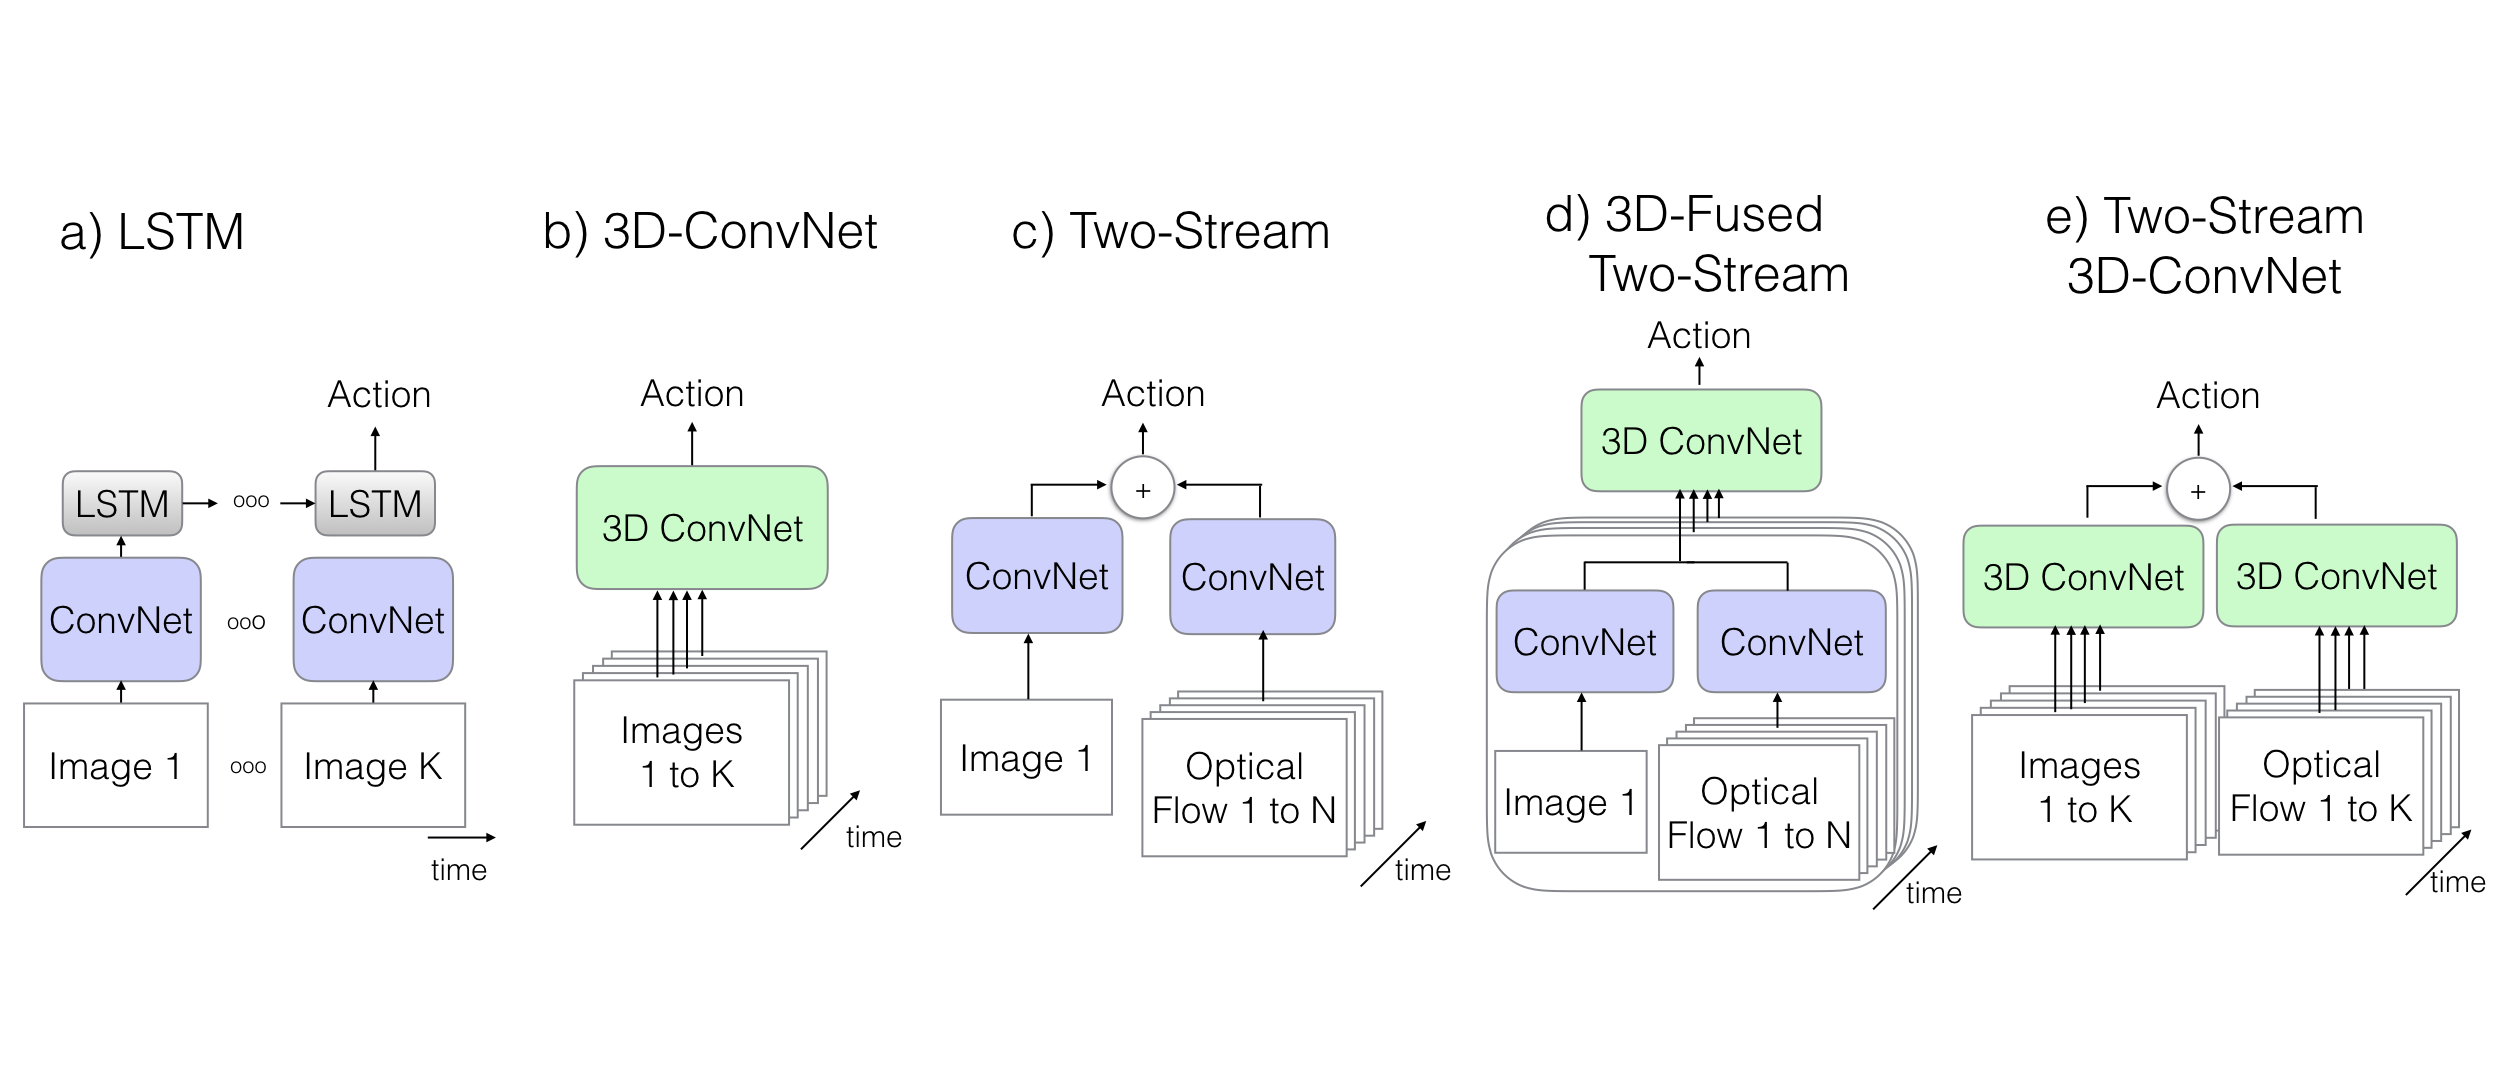
\includegraphics[width=1.0\textwidth]{assets/charts_rw/I3D}
    \caption[Illustration of Structures Discussed in I3D]{The structures discussed in the I3D paper, with subfigure (e) describingthe I3D structure itself. Source: \parencite{carreira2017quo}}
    \label{fig:structuresi3d}
\end{figure}

Some research suggests that optical flow may be replaced or improved due to the expensive computing resources used for its calculation. Such research has proposed networks to replace the pretrained optical flow model with architectures that inherently capture motion between frames or predict the optical flow in an end-to-end classification network. While these proposals are often more efficient in terms of computational resources and model parameters, they suffer from inferior performance \parencite{Lee_2018_ECCV, 8354283, Piergiovanni_2019_CVPR}.

\subsection{Pretext Learning}
Some more recent studies focus on designing different pretext tasks for the model to learn in a self-supervised manner \parencite{wang2022internvideo}.

With meticulous design, pretext learning can empower the model to produce high-quality visual representation within specific semantic spaces. These representations can further be employed in downstream tasks such as action recognition, video retrieval, or video captioning \parencite{10.1145/3577925}.

Some studies train models to predict appearance statistics \parencite{Wang_2019_CVPR}, rotation angles \parencite{DBLP:journals/corr/abs-1811-11387}, playback speed \parencite{Yao_2020_CVPR, 10.1007/978-3-030-58520-4_30}, and temporal order \parencite{10.1007/978-3-030-58604-1_26}. Another approach involves the design of contrastive learning models that determine whether two augmented images originate from the same source. Notable examples include MoCo \parencite{finn2017model} and SimCLR \parencite{pmlr-v119-chen20j}. The latter, SimCLR, processes two views augmented from a single image, and its objective is to maximize their similarity in the embedding space. These methodologies have been extended for application in the video domain \parencite{Feichtenhofer_2021_CVPR}.

Inspired by SimCLR, an Action Frame Contrastive Learning Network (AFRICAN) is proposed in this research to force the model to capture the fine-grained difference between frames in a video. In the pretraining stage of AFRICAN, frames in a video are augmented into two different views to do contrastive learning. The target of the contrastive learning model is to identify pairs of frames from the same frame source. This way, the model is able to explore weights that can capture the fine-grained difference between frames. 

\section{Backbone for Videos}
The Transformer architecture, originally introduced for machine translation \parencite{vaswani2017attention}, subsequently became a dominant model in the field of Natural Language Processing. Inspired by its success, the Vision Transformer (ViT) was proposed \parencite{dosovitskiy2020image}. Unlike the original Transformer, which was applied to one-dimensional sequences of text tokens, ViT segments an image into patches, and positional embeddings are added to each patch, thereby converting the image into a sequence of tokens.

Before the introduction of ViT, 3D Convolutional Neural Networks (3D CNN) were the standard backbone networks for extracting features from videos. Notable examples include C3D \parencite{tran2015learning}, I3D \parencite{carreira2017quo}, and Slowfast \parencite{feichtenhofer2019slowfast}. However, as the ViT was demonstrated to have superior theoretical and practical effectiveness, it began to be adopted as the primary backbone for video processing. A significant challenge for this shift is the computational cost. Despite the attention mechanism's impressive capabilities, it is notably resource-intensive.

Considering the temporal redundancy inherent in videos, the computation of attention could be reduced along the temporal axis. To this end, TimeSformer \parencite{bertasius2021space} was introduced, which computes key-query mappings solely for tokens that share specific spatial-temporal relationships. Subsequently, Uniformer \parencite{li2022uniformer} and its extension, Uniformer V2 \parencite{li2022uniformerv2}, were proposed to integrate the strengths of 3D CNN, good at extracting neighbouring features, with those of ViT, which efficiently maps the relationship between all tokens in a sequence. This hybrid structure proved to be an efficient video feature extractor, both reducing computational costs and enhancing performance. 

The subsequent subsections will elaborate on the mechanisms of Multi-Head Attention, ViT, TimeSformer, Uniformer, and its extension, Uniformer V2.


\subsection{Multi-Head Self-Attention}

\begin{figure}
    \centering
    \begin{subfigure}[b]{0.35\textwidth}
        \centering
        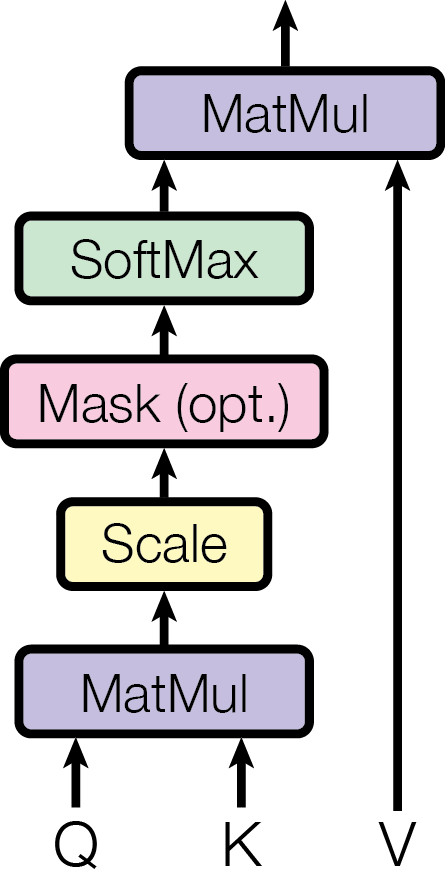
\includegraphics[width=\textwidth]{assets/charts_rw/Transformer_Attention.png}
        \caption{Scaled Dot-Product Attention}
        \label{fig:dotproductattention}
    \end{subfigure}
    \hfill
    \begin{subfigure}[b]{0.35\textwidth}
        \centering
        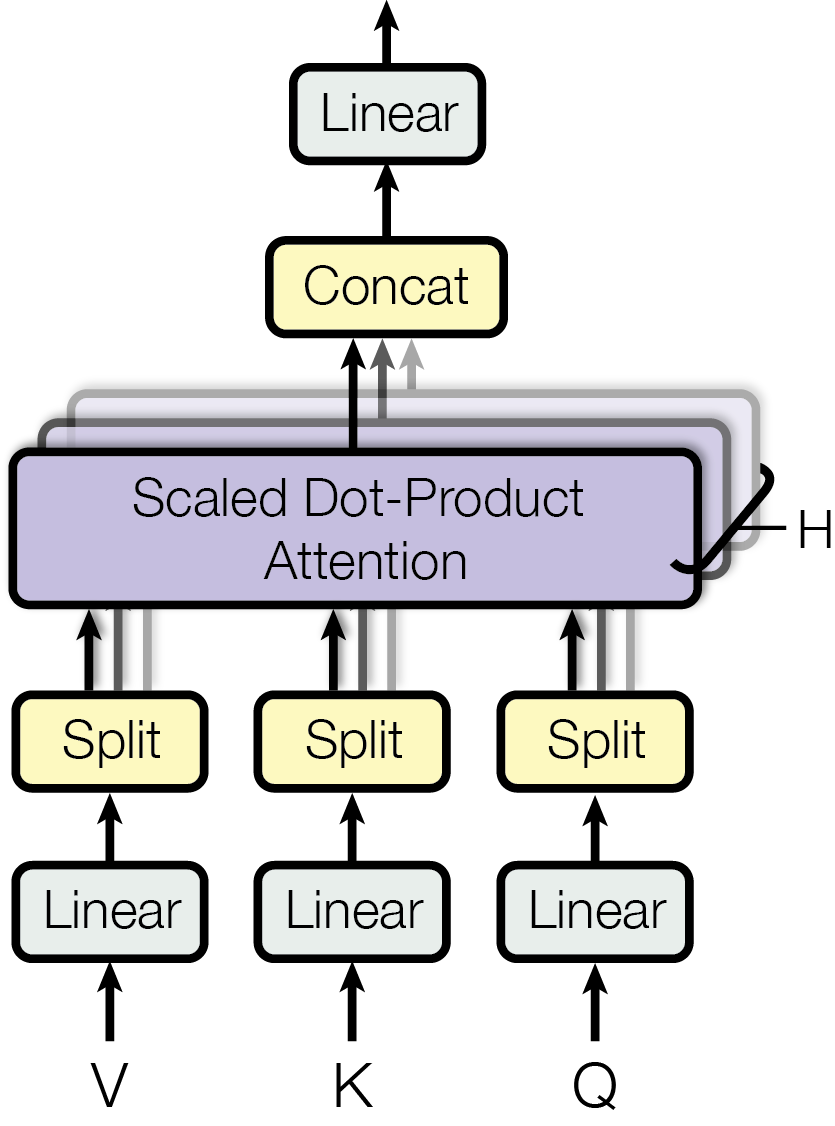
\includegraphics[width=\textwidth]{assets/charts_rw/Transformer_MultiHeadAttention.png}
        \caption{Multi-Head Attention}
        \label{fig:multiheadattention}
    \end{subfigure}
    \caption{Mechanisms of Scaled Dot-Product Attention and Multi-Head Attention. Source: \parencite{vaswani2017attention}}
    \caption{Mechanisms of Scaled Dot-Product Attention and Multi-Head Attention. Source: \parencite{vaswani2017attention}}
    
    \label{fig:attentionmechanism}
\end{figure}

For a clear introduction to ViT, understanding the Transformer's attention mechanism is pivotal. This process is visually described in Figure \ref{fig:attentionmechanism}. Given input data $X \in \mathbf{R}^{S \times d_k}$, where $S$ denotes the sequence length and $d_k$ stands for the embedding dimension, the initial step involves transforming the input vector using matrices $W_q \in \mathbf{R}^{d_k \times d_k}$, $W_k \in \mathbf{R}^{d_k \times d_k}$, and $W_v \in \mathbf{R}^{d_k \times d_k}$, producing three new vectors: query $Q \in \mathbf{R}^{S \times d_k}$, key $K \in \mathbf{R}^{S \times d_k}$, and value $V \in \mathbf{R}^{S \times d_k}$, as shown in the grey-shaded linear block of Figure \ref{fig:multiheadattention}.

These vectors, $Q$, $K$, and $V$ are then divided into $H$ heads, reshaping them to $(S, \frac{d_k}{H})$. The vectors for each head, specifically, $Q \in \mathbf{R}^{S \times \frac{d_k}{H}}$, $K \in \mathbf{R}^{S \times \frac{d_k}{H}}$, and $V \in \mathbf{R}^{S \times \frac{d_k}{H}}$ are then processed using the Scaled Dot-Product Attention, as illustrated in Figure \ref{fig:dotproductattention}. 

To calculate the attention score for tokens in a particular head, $Q$ and $K$ are multiplied together, scaled by the factor $\frac{1}{\sqrt{d_k}}$, and followed by a softmax function. The resulting matrix, $softmax\left(\frac{Q K^T}{\sqrt{d_k}}\right)$, having dimensions $(\frac{d_k}{H}, \frac{d_k}{H})$, represents the attention scores between all token pairs within that head. By multiplying this scores with $V$, the attention values, $\operatorname{Attention}(Q, K, V)$, of shape $(S, \frac{d_k}{H})$, are derived, as detailed in Equation \ref{eq:attentionscore}.
 
After obtaining the attention values for every head, they are concatenated to form the dimension $(S, d_k)$. This output is then passed through a feed-forward network to yield the final output of the Multi-Head Attention block.

\begin{equation}
    Attention(Q, K, V)=softmax\left(\frac{Q K^T}{\sqrt{d_k}}\right) V
    \label{eq:attentionscore}
\end{equation}

\subsection{Vision Transformer}

\begin{figure}[ht]
    \centering
    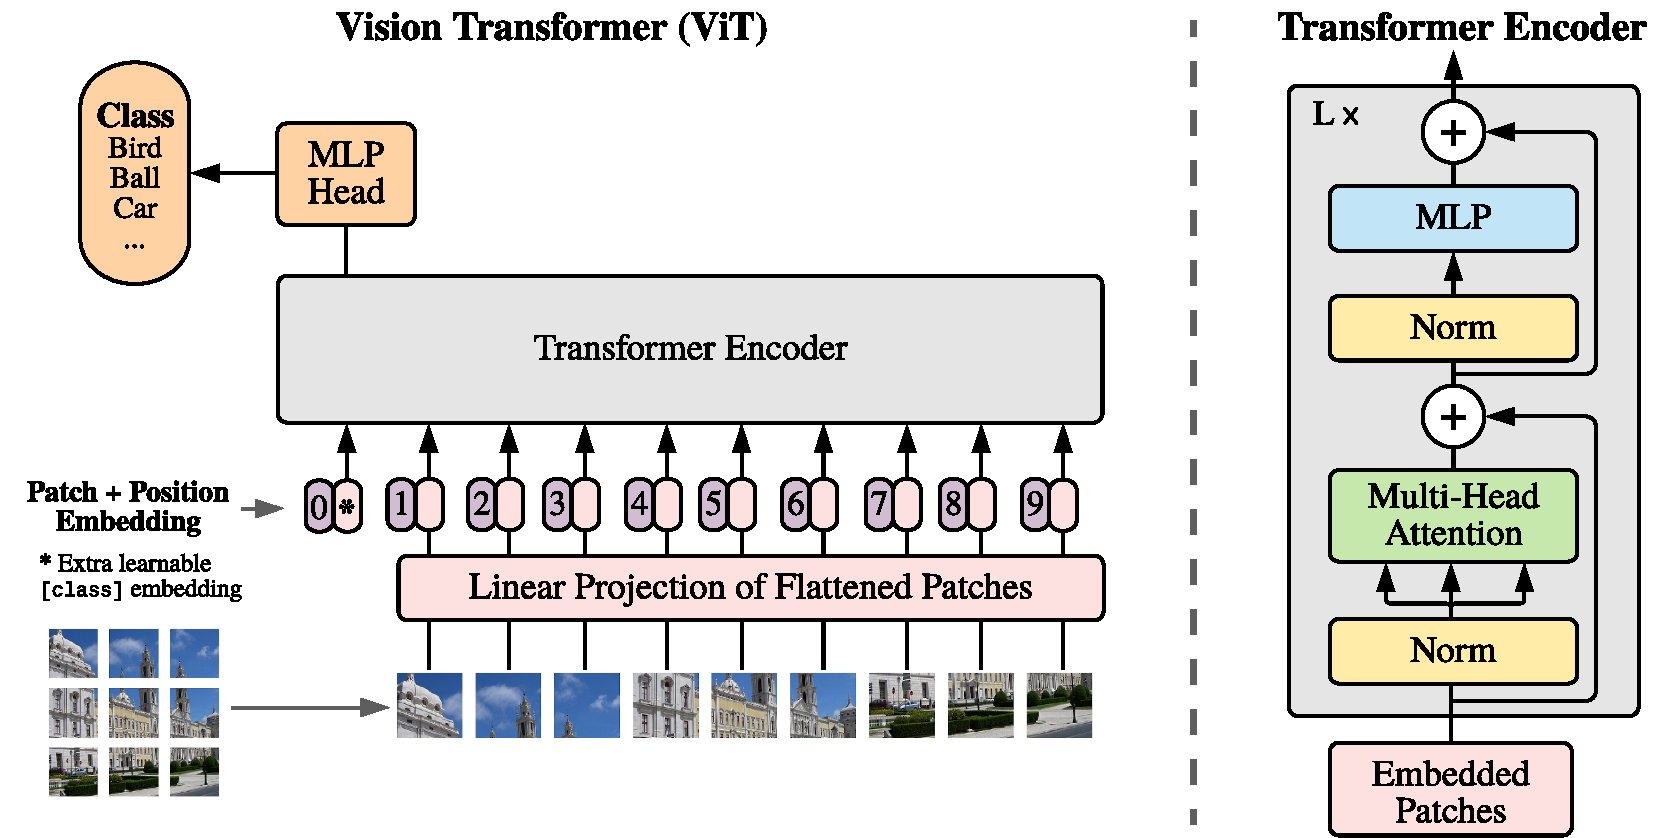
\includegraphics[width=1.0\textwidth]{assets/charts_rw/ViT}
    \caption[Illustration of ViT's Structures]{This figure illustrates the structures of ViT. Source: \parencite{dosovitskiy2020image}}
    \label{fig:structuresvit}
\end{figure}

The architecture of the Vision Transformer (ViT) for classification is illustrated in Figure \ref{fig:structuresvit}. To adapt an image for input into a standard Transformer, it is first divided into fixed-sized patches. Each patch is then flattened and linearly projected to produce embeddings. 

At the beginning of the sequence of embedded patches, a learnable $cls$ token (represented by $*$ in the figure) is inserted. This sequence of embeddings, including the $cls$ token, is then added with learnable positional embeddings, as indicated by the small purple blocks in the figure. Afterwards, the sequence is fed into the Transformer Encoder block. 

The Transformer Encoder, on the right side of the figure, is composed of $L$ consecutive layers. Within each layer, the processing steps contain two normalisation layers, a multi-head attention mechanism, two identity mappings, and a multi-layer perception (MLP) block. After processing through the Encoder, the final MLP head operates on the $cls$ token to produce logits for each classification category.

\subsection{TimeSformer}
\begin{figure}[ht]
    \centering
    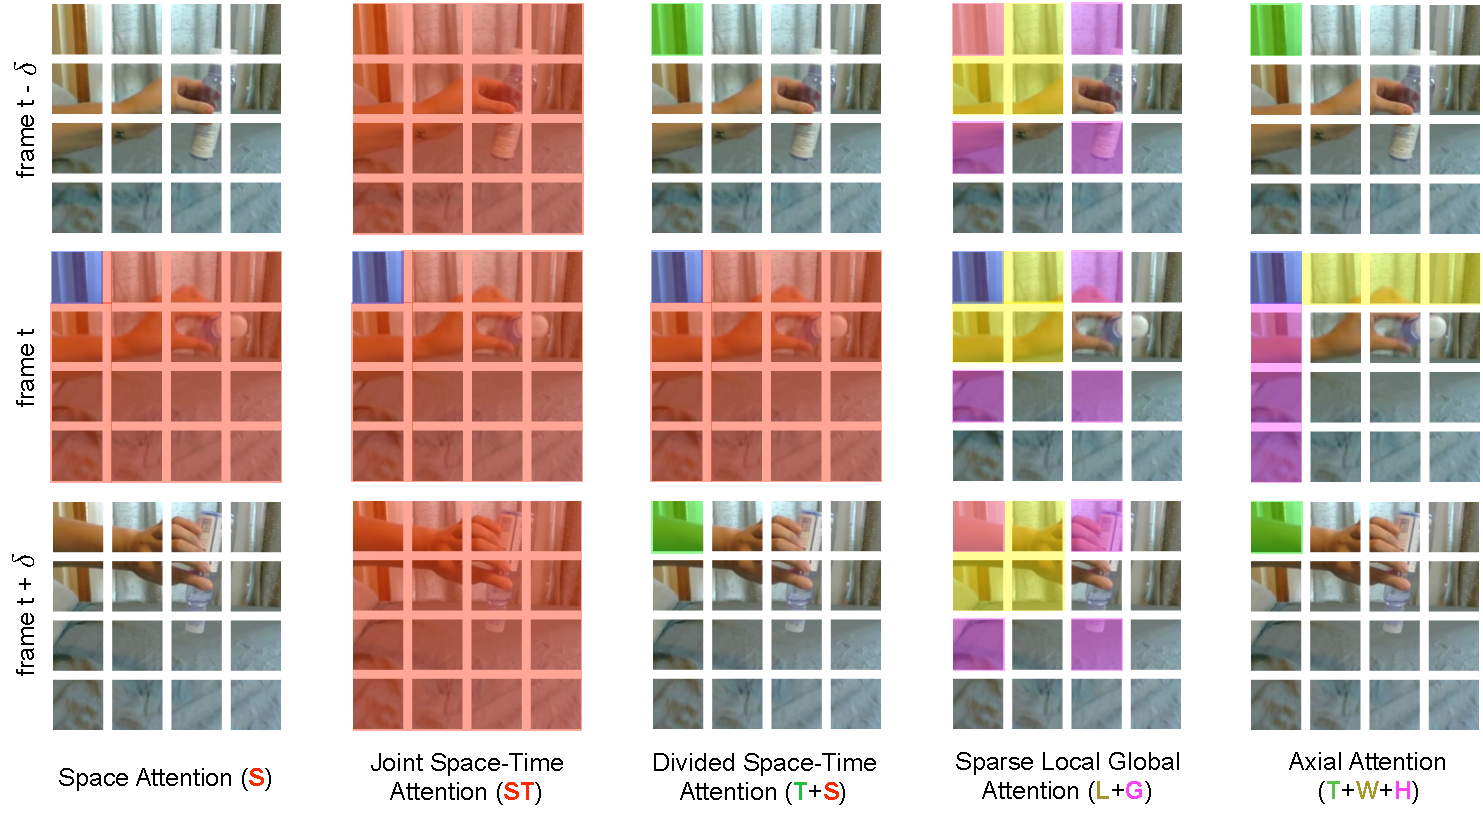
\includegraphics[width=1.0\textwidth]{assets/charts_rw/Timesformer}
    \caption[Five different space-time attention schemes studied by TimeSformer]{Illustration of the five different space-time attention schemes studied by TimeSformer. Source: \parencite{bertasius2021space}}
    \label{fig:structurestimesformer}
\end{figure}

Adapting the image transformer to process videos introduces a critical challenge: computational expense. Unlike images, videos inherently possess a spatio-temporal nature, adding an additional dimension, which exponentially increases the size of input data. This complexity makes it computationally intensive to implement an attention mechanism across all patches split from all frames within a video.

To address this challenge, TimeSformer introduces an innovative approach to managing the spatio-temporal dynamics of videos. Rather than directly applying the attention mechanism to both spatial and temporal dimensions, the model investigates five different space-time attention strategies. As illustrated in Figure \ref{fig:structurestimesformer}, among these strategies, the Divided Space-Time Attention outperforms the others to be the most efficient and effective approach.


\subsection{Uniformer and Uniformer V2}
\begin{figure}[ht]
    \centering
    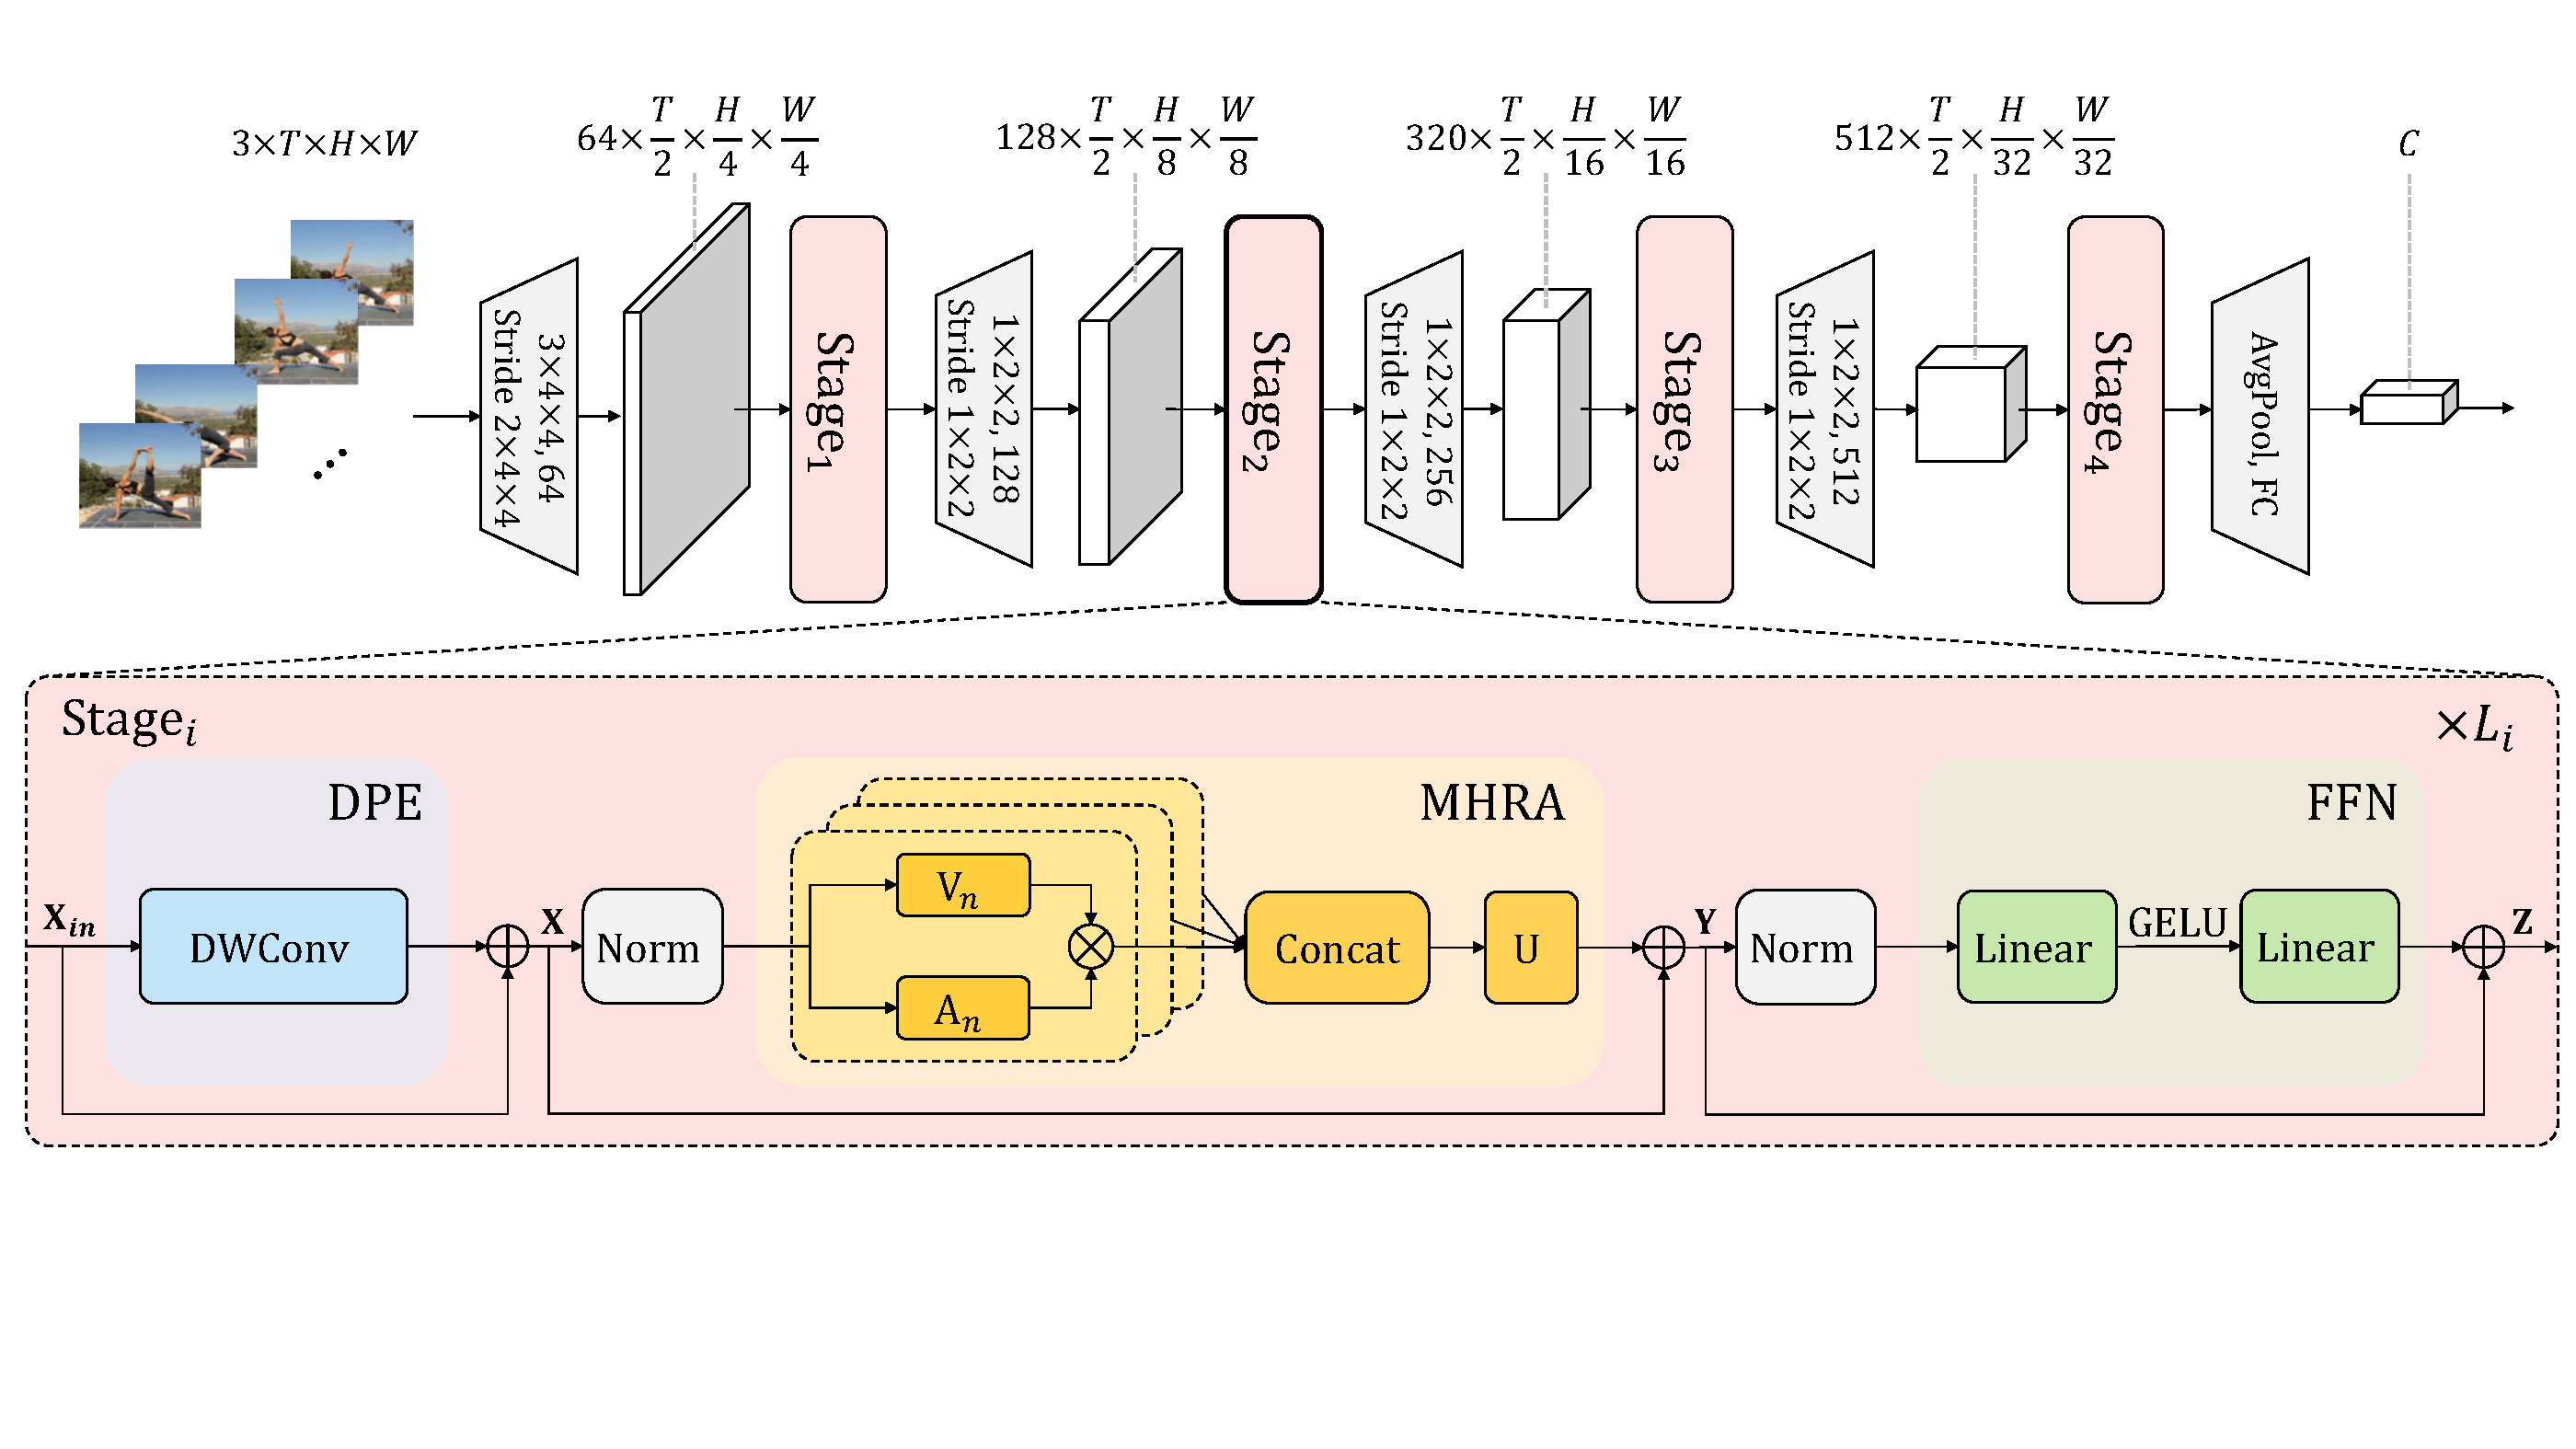
\includegraphics[width=1.0\textwidth]{assets/charts_rw/Uniformer}
    \caption[The Structure of Uniformer]{Illustration of the structure of Uniformer. Source: \parencite{li2022uniformer}}
    \label{fig:structureuniformer}
\end{figure}

Uniformer combines the strengths of the ViT and 3D CNN for video feature extraction. While ViT excels in identifying global relationships between distant tokens, 3D CNN is good at capturing local attention patterns between adjacent tokens. Nonetheless, instead of solely relying on the 3D CNN for local feature extraction, Uniformer introduces a Unified Transformer designed to mimic the functionality of the 3D CNN in this aspect.

Figure \ref{fig:structureuniformer} displays the architecture of Uniformer, segmented into four distinct Uniformer blocks. Each block consists of the Dynamic Position Embedding (DPE), Multi-Head Relation Aggregator (MHRA), and Feed Forward Network (FFN) modules:

\begin{itemize}
    \item \textbf{DPE}: This module employs a combination of absolute and relational embeddings, overcoming the various lengths of video frames while preserving crucial positional information.
    \item \textbf{MHRA}: MHRA aggregates each token with its contextual tokens. Specifically, it utilizes the Unified Transformer to calculate the attention of embeddings within a $t\times{h}\times{w}$ tube in the shallow layers. As it progresses to the deeper layers, it broadens its scope, applying global attention to all tokens.
    \item \textbf{FFN}: A feed-forward network composed of two linear layers and a GELU layer.
\end{itemize}

\begin{figure}[ht]
    \centering
    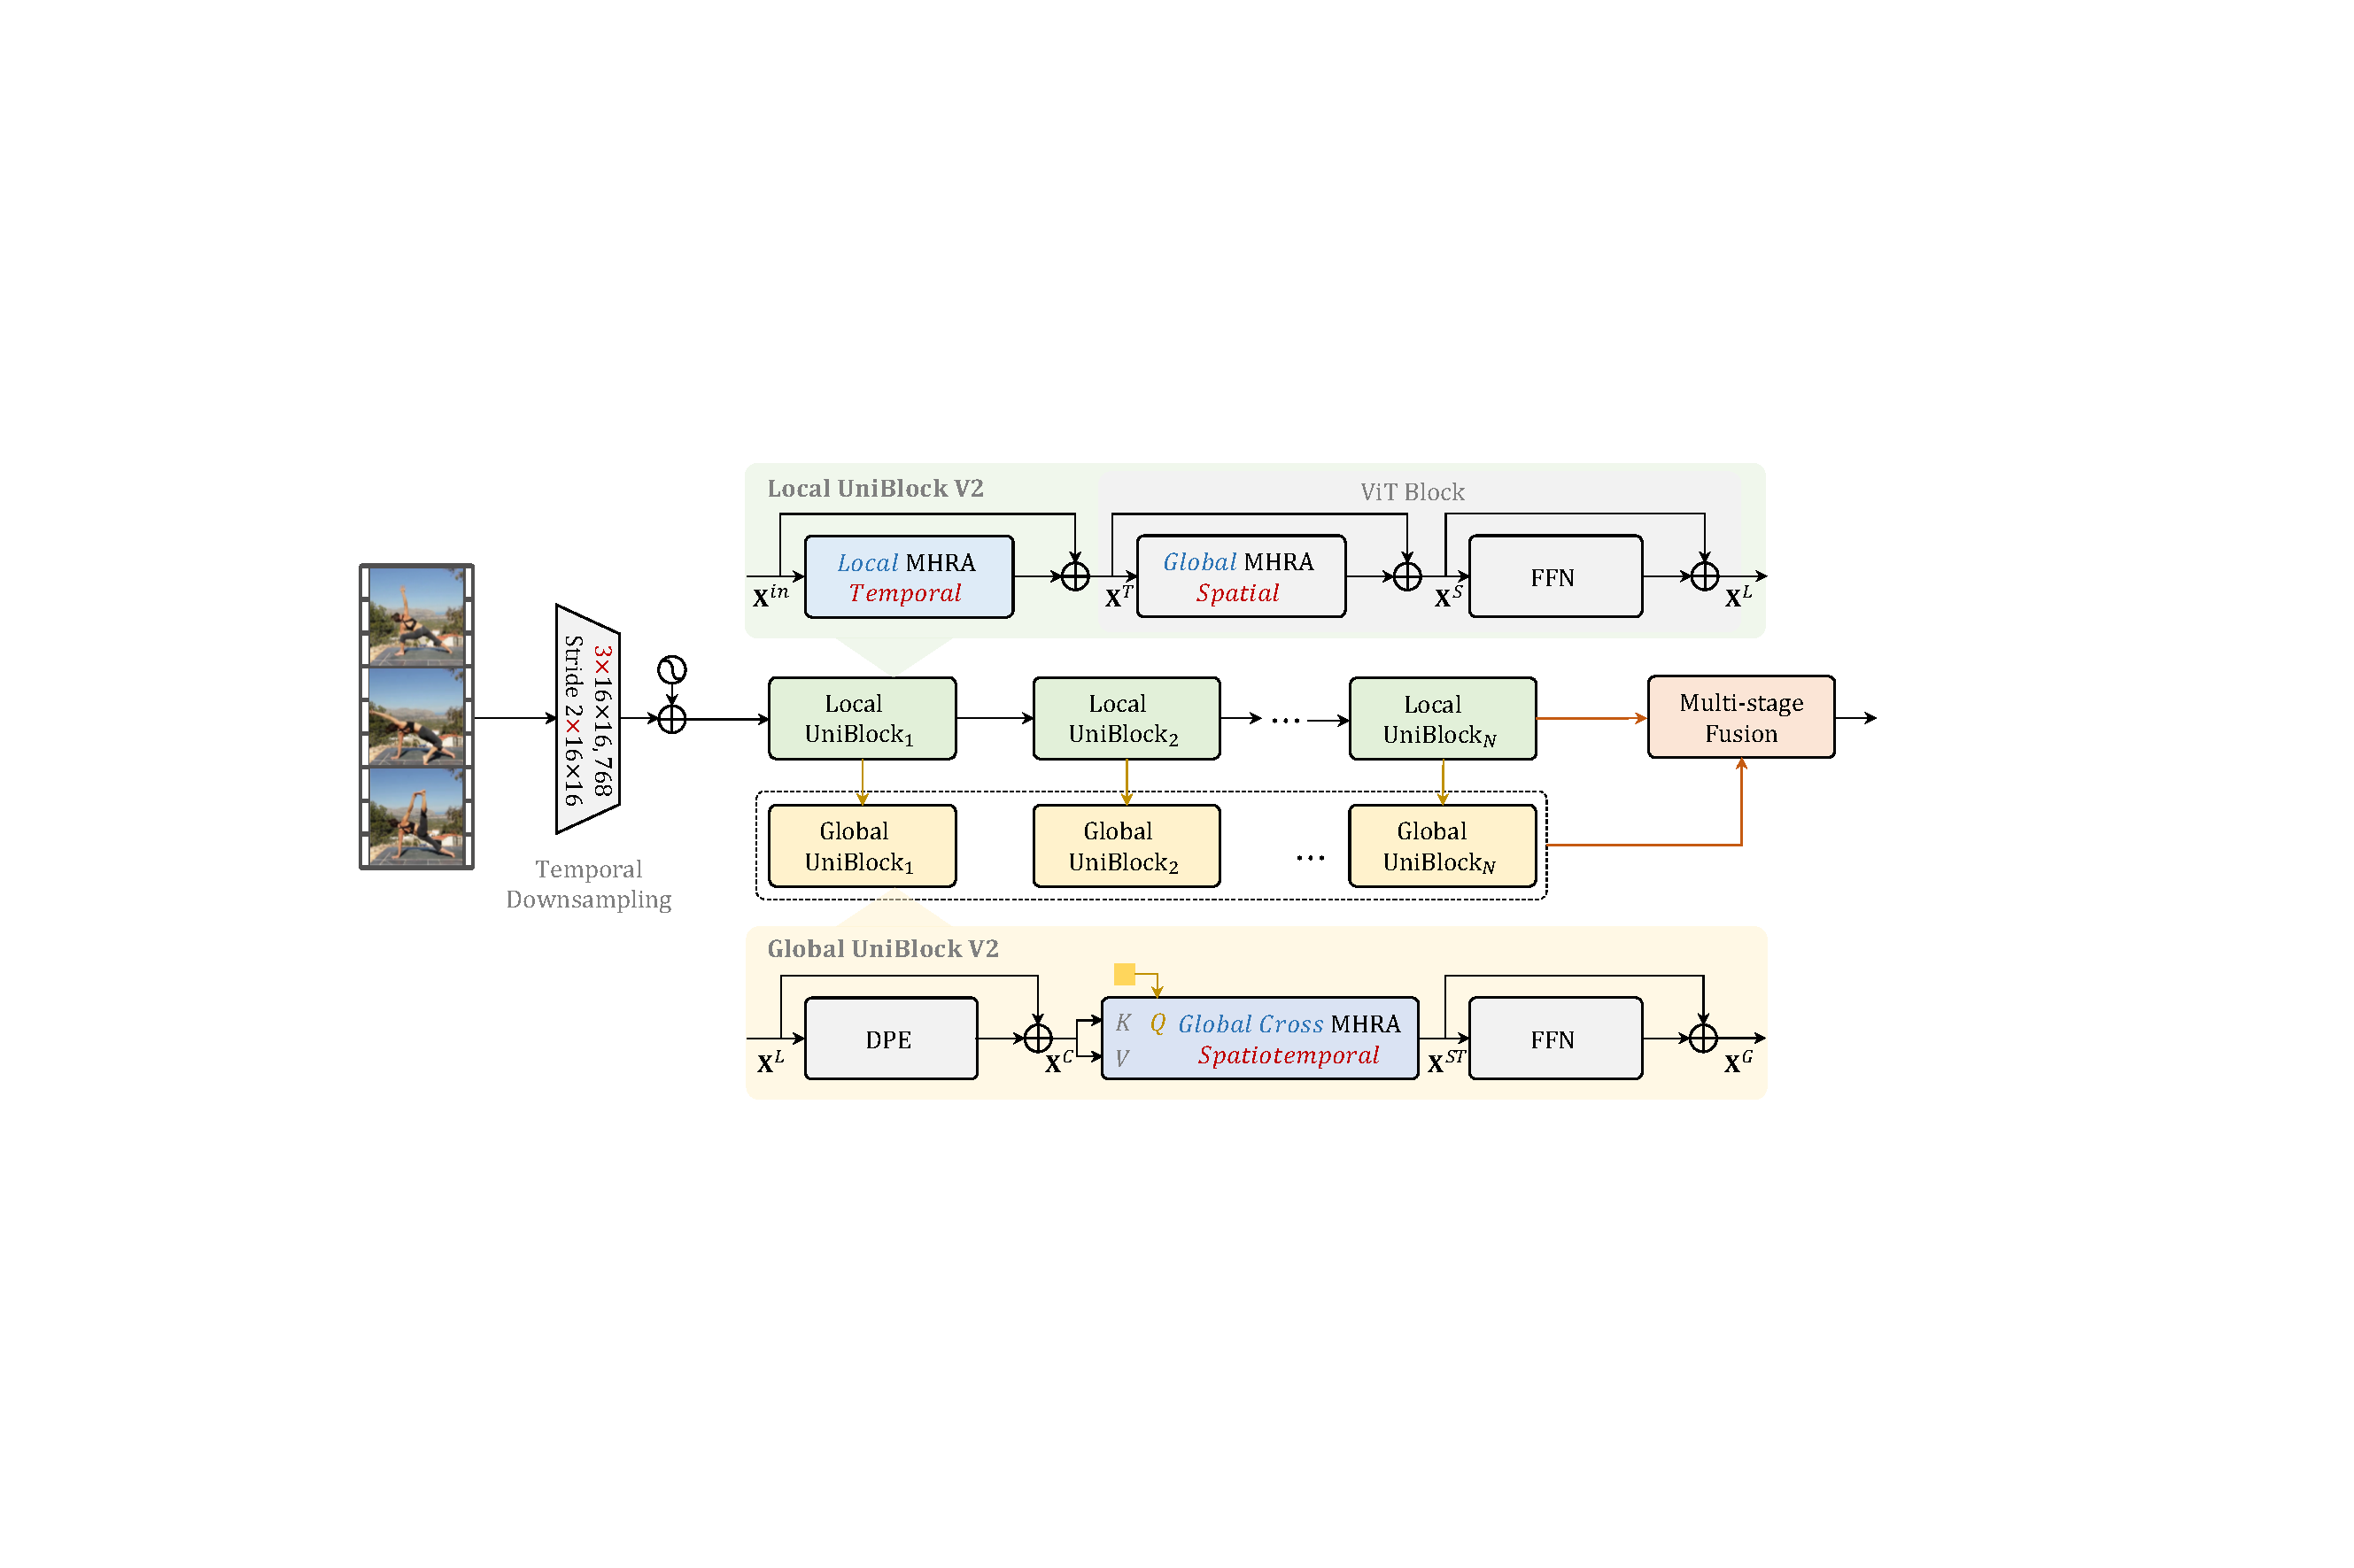
\includegraphics[width=1.0\textwidth]{assets/charts_rw/UniformerV2}
    \caption[The Structure of Uniformer V2]{Illustration of the structure of Uniformer V2. Source: \parencite{li2022uniformerv2}}
    \label{fig:structureuniformerv2}
\end{figure}

As shown in Figure \ref{fig:structureuniformerv2}, Uniformer V2 is composed of a sequence of Local Unibolck V2 and Global Uniblock V2. Each Local Unibolck V2 contains a Local Temporal MHRA (denoted as LT\_MHRA), a Global Spatial MHRA (GS\_MHRA), and an FFN. The LT\_MHRA applies the attention mechanism on every $t\times1\times$ tube in a video, while the GS\_MHRA functions as the original ViT Block. The FFN includes two linear layers and a GELU layer. 

In contrast, each Global Uniblock V2 contains a DPE layer, a Global Cross Spatial attention MHRA (C\_MHRA), and an FFN. The DPE layer and FFN has been introduced in the previous section. The core operation of C\_MHRA is cross attention. 

Different from self-attention, in cross-attention, the query, key, and value are from different sequences. C\_MHRA employs the cls token, the first token of the sequence, as the query, and the subsequent patch embeddings serve as the key and value, computing the video embedding. This well-designed model has been the first model to achieve 90.0\% top-1 accuracy on the Kinetics-400 \parencite{kay2017kinetics} dataset, which is one of the most notable datasets in action recognition. As a consequence, this model is selected as the research backbone.

\section{Vision-Text Contrastive Learning}
Vision-text contrastive learning has marked a significant advancement in the computer vision domain. Because these models are trained to embed visual and textual data into a shared semantic space, they are able to understand visual content in terms of human language, a well-defined knowledge system developed by humans. 

This most notable example of vision-text contrastive learning is Contrastive Language-Image Pre-training (CLIP) \parencite{radford2021learning}. As it utilises a large amount of image-captioning data, including pre-existing datasets and web-crawled data, to train both an image and text encoder, they are able to encode the images and the text into a common semantic space for subsequent analyses. To adapt this to videos, InternVideo modified the visual encoder's backbone \parencite{wang2022internvideo} based on their prior work, Uniformer V2.

Subsequent sections will explain the mechanism of CLIP in detail.

\subsection{Contrastive Language-Image Pre-training (CLIP)}
\begin{figure}[ht]
    \centering
    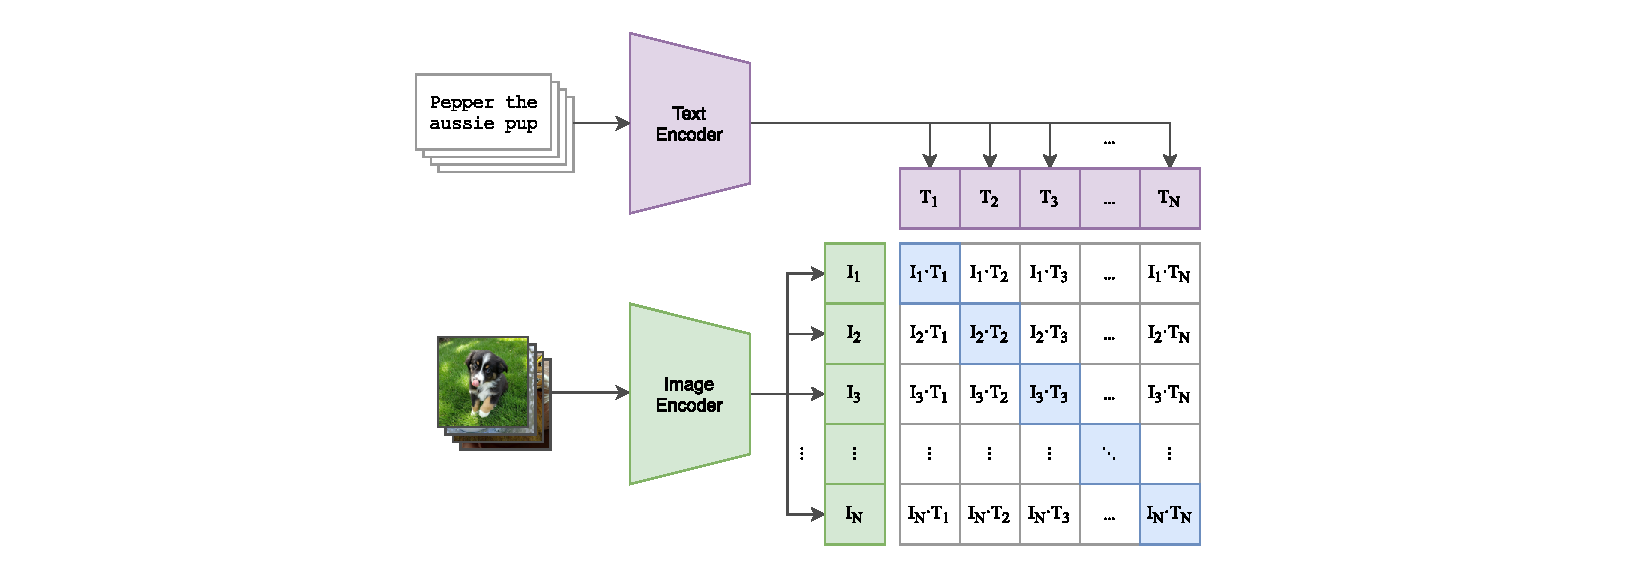
\includegraphics[width=1.0\textwidth]{assets/charts_rw/CLIP_loss}
    \caption[Training Structure of CLIP]{Illustration of the CLIP training structure. Source: \parencite{radford2021learning}}
    \label{fig:cliplossstructure}
\end{figure}

Figure \ref{fig:cliplossstructure} illustrates the training structure of CLIP. The inputs for the model include an image and its corresponding caption, both of which are encoded into embeddings. To derive the similarity matrix $S$ illustrated in the figure, the dot product method, combined with a scaling factor, is applied as demonstrated in Equation \ref{eq:clipsimilarity}. 

\begin{equation}
    \label{eq:clipsimilarity}
    S = (IE \cdot TE^T) \times exp(t)
\end{equation}

where $\mathbf{IE} \in \mathbb{R}^{B \times E}$ represents the image embeddings and $\mathbf{TE} \in \mathbb{R}^{B \times E}$ represents the text embeddings in a training batch. $B$ is the batch size, $E$ is the embedding dimension, and $t$ is a trainable scale factor. Through this equation, the model is optimised to identify correct image-text pairs, achieving high similarity scores for accurate pairs while minimizing scores for incorrect pairs. The InfoNCE loss \parencite{oord2019representation}, a variant of the categorical cross-entropy, is used for model optimisation.

\begin{equation}
    \label{eq:infonce}
    InfoNCE_q = -log \frac{exp(q \cdot k_+ / \tau)}{\sum_{i=0}^{k}{exp(q \cdot k_i / \tau)}}
\end{equation}

This equation calculates the InfoNCE loss for a specific query $q$, which is the embedding of a given image, where $k_+$ denotes the positive key, meaning the correct or corresponding text for the image, and $k_i$ denotes all the keys including positive and negative Examples. 

$\tau$ is a temperature parameter that scales the logits before applying the softmax. This parameter can adjust the smoothness of the input logits: a larger $\tau$ narrows the range of input logits, while a smaller $\tau$ increases the scale of the logits. The narrower range of input logits suggests equally calculating the loss affected by negative samples, while the amplified scale of the logits leads to the exponential marginal effect of the negative sample's logit.

% \subsection{Video CLIP module in InternVideo}

